% Study 1 report. Compile with pdflatex + bibtex (plainnat) on TeX Live or MiKTeX.
% Every number traces to a file and a command listed in sources.md and asserted by check_numbers.py.
\documentclass[10pt]{article}
\usepackage[a4paper,margin=24mm]{geometry}
\usepackage{amsmath}
\usepackage{booktabs}
\usepackage{graphicx}
\usepackage[hyphens]{url}
\usepackage[numbers,sort&compress]{natbib}
\usepackage[colorlinks=true,allcolors=blue]{hyperref}

\graphicspath{{figures/}}
\newcommand{\lm}{\texttt{local\_mean\_28}}
\newcommand{\aets}{\texttt{autoets\_weekly}}
\newcommand{\qs}{QScore9}
% DOI: the author reserves the DOI on posting day and replaces the text below.
\newcommand{\reportdoi}{DOI to be filled on posting day}

\title{Zero-shot foundation models on sparse daily GitHub star counts:\\a registered re-evaluation after an audit}
\author{Victor Prchlik}
\date{Report version, October 2026 \\ \small \reportdoi}

\begin{document}
\sloppy
\maketitle

\begin{abstract}
We revisit whether zero-shot time-series foundation models improve probabilistic forecasts of daily GitHub
star counts. A first version found Chronos-2 and TimesFM-2.5 ahead of four classical baselines on mean CRPS
in every cell. An audit found no invalidating code defect but two design flaws: cohorts selected on outcomes
unavailable at forecast time, and evaluation windows dominated by post-peak decay. We pre-registered a
redesign (protocol commit \texttt{5f01769}, 2026-09-12) and ran it unchanged: from 148,550 repositories
created 2023-01-01 to 2025-02-21 with at least 20 archived stars in their first 90 days, 300 sampled by a
seeded rule in three day-90 activity strata; daily counts from GitHub's star-history endpoint through
2026-08-31; three non-overlapping trailing cutoffs, horizons of 7, 30 and 90 days; three frozen models
(Chronos-2, TimesFM 3, TimesFM 2.5) against a 28-day local mean and weekly AutoETS; a nine-decile quantile
score with repository-clustered inference, 18 declared comparisons. Against the local mean the mean
difference favors the models in every cell and its bootstrap interval excludes zero in five of nine, but the
typical repository favors the reference: the models score lower on 46 to 89 of 300 repositories and the
signed-rank test rejects in all nine cells on the reference's side. Against AutoETS both summaries favor the
models, the mean in all nine cells and the win count on 293 to 298 of 300, consistent with its 80 percent
intervals covering about 99 percent of target days. A post-hoc accounting locates the mean gain on positive
days where the local mean overpredicts; the zero-day part is small beside it. The registered second study,
the registered follow-up cohort and the lapsed prospective holdout are stated as not run.
\end{abstract}

\section{Introduction}

The question is whether zero-shot time-series foundation models improve probabilistic forecasts of the daily
number of new stars a GitHub repository receives. These series are counts, most days are zero for most
repositories, activity arrives in bursts tied to releases and external attention, and the panel one can
observe is survivor-biased: a repository that was deleted or made private has no history to fetch. Public
forecasting benchmarks are mostly smooth, seasonal, positive series, so this kind of data is a hard case for
zero-shot forecasting. The practical question is whether such a model is worth running at all on a sparse
count series, or whether a trailing mean does as well.

The story of this report is in four parts. A first version of the study, built in June and July 2026, found
two foundation models ahead of classical baselines on mean CRPS in every cell of its design. An adversarial
audit on 2026-07-12 found no code defect that invalidated the aggregate comparison, but two design flaws that
could not be fixed by rewriting prose: the cohorts had been selected on outcomes not available at forecast
time, and the evaluation windows mostly tested post-peak decay. We registered a redesign on 2026-09-12, before
any target was fetched, and ran it on 2026-09-13 without change. The revised result is less flattering and is
reported with the same care: the models win on the mean against a 28-day local mean, lose on most individual
repositories, and win on both summaries against a weekly AutoETS whose intervals are far too wide. A post-hoc
accounting of the saved run, labeled as such, says where the mean gain comes from.

This is not the first observation that an aggregate gain can coexist with a minority win rate. A July 2026
quick-commerce study found TimesFM's pooled gains concentrated in high-turnover items while it won a minority
of item-rounds on lumpy demand \citep{kim2026}, and a marketplace-panel study showed the aggregate and
per-series rankings of five zero-shot foundation models reversing on M5 \citep{islam2026}. Frozen foundation
models have also been evaluated on sparse daily counts before: twelve of them, the three used here among
them, on five sparse panels as an event-ranking task without a proper score \citep{schoess2026}; and TimesFM 3
on simulated intermittent demand, where its nine-decile pinball loss was no better than the history's
empirical deciles \citep{ebrahim2026}, a finding consistent with the typical-repository result reported here.
Earlier evaluations on cloud workloads found simple baselines ahead \citep{toner2025}, and the Chronos and
TimesFM papers themselves report benchmark results that include count-like series without a zero-day
diagnosis \citep{ansari2024, das2023}. Benchmark practice has moved toward reporting win rates alongside
relative errors \citep{fevbench2026}, and the forecast-evaluation literature warns against ratio metrics that
silently drop series \citep{hewamalage2023}. Star-count prediction on GitHub has been studied as a regression
on popular repositories \citep{borges2016}, and a live benchmark scores daily new stargazers on the 400
most-starred repositories \citep{garza2026}; the present design samples from a population rather than from
the popular. What this report adds is a registered, population-sampled, repository-clustered probabilistic
evaluation whose every number traces to a saved file.


\section{Version 1 and the audit}

Version 1 ingested 208 repositories found by three GitHub Search API queries (recently created and already
high-starred; old, moderate and recently maintained; not pushed in years), giving 414,271 daily rows from
2008-11-13 to 2026-06-22, of which 179 repositories had at least 270 days of history (41, 69 and 69 in the
three cohorts). The backtest used an expanding context starting 180 days after the first star, a 30-day step,
at most eight windows per repository, horizons of 7, 30 and 90 days, and 200 predictive trajectories per
model. Four classical baselines (horizon-dependent seasonal naive, linear trend, damped ETS, LightGBM) and two
foundation models, Chronos-2 and TimesFM-2.5, were scored by empirical CRPS. Both foundation models had lower
mean CRPS than every original baseline in all nine cohort-by-horizon cells; in the ``breakout'' cohort the
foundation models scored 6.2 to 8.5 against 11.2 to 28.0 for the baselines.

The audit of 2026-07-12 found no code defect that invalidated the aggregate six-model comparison; every
summary field recomputed from the saved artifact. It found two design flaws that invalidated the original
claims:
\begin{enumerate}
\item \emph{Outcome-conditioned cohorts.} ``Breakout'' was selected for already having many stars, ``dead''
  for later inactivity, ``steady'' for later maintenance. None of these labels was available at forecast
  time. The ``dead'' cohort's evaluation windows had a median of 5.02 stars per day and only 7.7 percent zero
  days; it was not dead when evaluated.
\item \emph{Post-peak windows.} The global peak preceded the evaluated span for 78.0 percent of breakout
  repositories; only 12.2 percent peaked inside it. The study tested the forecasting of post-viral decay, not
  of shocks.
\end{enumerate}
After the audit added a 28-day local mean on identical windows, the foundation models still had the lower
mean in every cell (Appendix Table~\ref{tab:v1}), but the per-repository win rate against it fell to between
40.6 and 80.5 percent, and the audit put the share of positive gain held by the five largest positive
contributors at roughly 30 to 77 percent depending on the cell, a figure it tied to no named reference. The
audit also listed what version 1 had to disclose (Appendix~\ref{app:v1}). Its prescription, freeze and
pre-register, context-only labels, trailing non-overlapping windows with a common endpoint, strong
pre-registered baselines, native quantile metrics, repository-clustered inference, and a prospective
post-release cohort as the contamination control, became the specification of version 2; the cohort is
registered and not yet run (Section~\ref{sec:notrun}). Every version 1 number in this report is quoted from
the preserved version 1 documents, not recomputed; the version 1 artifacts are on a computer the author no
longer uses.


\section{The registered design}

The protocol was registered at commit \texttt{5f01769b6be4c32814befdd7cc3395b6dcc386ed} on 2026-09-12,
before any target history was fetched; the registered file's SHA-256 is
\texttt{dfe2f4adf5c3fdafaa6f2716ae7c19cd4d52577497041c13b763ba06540f65c5}. The run's gate verified those
exact bytes. Nothing in the protocol changed after results were seen; later changes are dated additions at its
end. What follows is the design in brief; Appendix~\ref{app:design} gives the count source and its
validation, the calendar, the regime rules, the model pins, the score and the inference settings as
registered.

The question is whether zero-shot foundation models improve probabilistic forecasts of daily GitHub
star-history counts relative to \lm{} and weekly AutoETS on a panel selected by day-90 activity and
fetch-time availability; the hypothesis predicts lower repository-level \qs{} for the foundation models, and
null, adverse, mixed and imprecise results receive the same reporting. The frame is every repository created
from 2023-01-01 to 2025-02-21 (UTC) with at least 20 GH Archive WatchEvents over the creation day and the
following 89 days, in three day-90 strata (20 to 99, 100 to 999, at least 1,000 events). Within each stratum
the frame is placed in a seeded random order (selection seed 20260913), frozen before retrieval; the walk
stops at 100 repositories with complete retrieved histories, with every skip and its reason logged, and
acceptance depends on retrieval completeness only. Daily counts come from GitHub's star-history endpoint,
from creation through the common endpoint 2026-08-31, binned to America/Los\_Angeles days after an hourly
validation against GH Archive; the target is the surviving-star daily history as retrieved in September
2026. Three cutoffs, 2025-12-05, 2026-03-05 and 2026-06-03, partition the trailing 270 days into
non-overlapping 90-day windows; horizons of 7, 30 and 90 days share each cutoff. Three context-only regime
labels are descriptive. Three frozen foundation models at pinned revisions (Chronos-2, TimesFM 3, TimesFM
2.5) are compared with two primary references, \lm{}, the mean of the last 28 context days with empirical
context-level draws, and \aets{}, AutoETS with season length 7 and native intervals; thirteen secondary
baselines add no test. The score is \qs{}, twice the mean pinball loss over the nine deciles and the target
days, a proper score for the nine quantiles. Window scores are averaged within repository and horizon,
repositories are weighted equally, and each of the 18 declared comparisons (three models, two references,
three horizons) reports the mean paired difference with a repository-bootstrap interval, the median
difference and a two-sided Wilcoxon signed-rank test, with one Benjamini-Hochberg adjustment at $q = 0.05$
over the 18 tests.


\section{The achieved panel}

The frame held 148,550 eligible repositories: 100,687 in the 20 to 99 stratum, 46,811 in 100 to 999, and
1,052 in the 1,000-plus stratum (Table~\ref{tab:panel}). The seeded walk accepted 100 per stratum and skipped
470 repositories, all because the stable ID no longer resolved to a public repository at fetch time (466 with
HTTP 404) or was forbidden (4 with HTTP 403). The panel is therefore repositories still public in September
2026 with complete retrievable histories; equal repository weighting describes this panel, not all of GitHub.
The daily signal holds 289,316 repository-days with every Los Angeles calendar day from creation through
2026-08-31 observed; no missing bin was imputed. The panel is evaluated in its mature phase: the creation
dates run from 2023-01-02 to 2025-02-19, so every repository was created at least nine months before the
first cutoff, and nothing here is a launch forecast.

\begin{table}[t]
\centering\footnotesize
\caption{The achieved panel by day-90 stratum: the frame size, the accepted and skipped counts, the median
and the 10th and 90th percentiles of the survivor ratio, the number of repositories with no star from
2026-06-03 to 2026-08-31, and the median star count over those 90 days. The survivor ratio divides the
endpoint's first 90 Los Angeles days by the gross archive count over the UTC creation day and the next 89
days; the two calendars differ, so the ratio is a diagnostic, not an exact retention rate. Skips are
repositories encountered before the stratum's stop.}
\label{tab:panel}
\begin{tabular}{lrrrrrrrr}
\toprule
Stratum & Frame & Accepted & Skipped & Ratio median & P10 & P90 & Zero, last 90 & Median, last 90 \\
\midrule
20--99 & 100,687 & 100 & 98 & 0.968 & 0.723 & 1.075 & 52 & 0 \\
100--999 & 46,811 & 100 & 348 & 1.004 & 0.885 & 1.079 & 22 & 4 \\
1000+ & 1,052 & 100 & 24 & 1.006 & 0.914 & 1.049 & 1 & 39 \\
\bottomrule
\end{tabular}
\end{table}

Over the 900 repository-cutoff windows, the context-only regime labeler assigned 320 windows from 140
repositories to ``inactive recently'', 572 windows from 228 repositories to ``other active'', and 8 windows
from 7 repositories to ``recent surge''. The surge regime is too thin to say anything about bursts, and the
report does not try.

The registered run started 2026-09-13 07:54 UTC at implementation commit
\texttt{ca67dd22ea49377ee1fd074aed57b4b7460c84f1} after the signed readiness review, and completed in
18,662 seconds (5 hours and 11 minutes) with 48,600 forecast rows (300 repositories, 3 cutoffs, 3 horizons,
18 models), no failed window and no resume. The integrity check recomputed every score and verified all 300
checkpoint hashes.


\section{Results}
\label{sec:results}

Tables~\ref{tab:lm} and~\ref{tab:ae} give the 18 declared comparisons, one table per reference, each with the
mean difference and its interval, the median difference, the number of repositories where the model's \qs{}
is lower, the strict win fraction and the adjusted $p$-value side by side. Figure~\ref{fig:paired} shows the
same. The two summaries, the mean and the typical repository, are always shown together because they
disagree.

\begin{table}[t]
\centering\small
\caption{The nine declared comparisons against \lm{}. Differences are model minus reference \qs{}, averaged
over three windows within repository and then over 300 repositories; negative favors the model. The interval
is the pointwise 95 percent percentile interval from 20,000 repository-cluster bootstrap replicates. ``Lower''
counts repositories (of 300) where the model's score is strictly lower; the strict win fraction divides by
300. $p$ is the Benjamini-Hochberg adjusted two-sided Wilcoxon signed-rank $p$-value over the 18 tests.}
\label{tab:lm}
\begin{tabular}{llrcrrrr}
\toprule
Model & $h$ & Mean & 95\% interval & Median & Lower & Win fraction & Adjusted $p$ \\
\midrule
Chronos-2 & 7 & -0.137 & [-0.342, 0.009] & 0.0010 & 79 & 0.263 & $1.0 \times 10^{-5}$ \\
Chronos-2 & 30 & -0.132 & [-0.285, -0.022] & 0.0018 & 59 & 0.197 & $5.5 \times 10^{-12}$ \\
Chronos-2 & 90 & -0.101 & [-0.211, -0.016] & 0.0023 & 50 & 0.167 & $1.4 \times 10^{-13}$ \\
TimesFM 3 & 7 & -0.258 & [-0.718, 0.012] & 0.0003 & 89 & 0.297 & $6.7 \times 10^{-3}$ \\
TimesFM 3 & 30 & -0.201 & [-0.488, -0.024] & 0.0004 & 75 & 0.250 & $8.4 \times 10^{-7}$ \\
TimesFM 3 & 90 & -0.128 & [-0.296, -0.016] & 0.0032 & 54 & 0.180 & $6.4 \times 10^{-12}$ \\
TimesFM 2.5 & 7 & -0.243 & [-0.695, 0.025] & 0.0015 & 68 & 0.227 & $3.2 \times 10^{-8}$ \\
TimesFM 2.5 & 30 & -0.201 & [-0.510, -0.015] & 0.0028 & 49 & 0.163 & $2.4 \times 10^{-13}$ \\
TimesFM 2.5 & 90 & -0.112 & [-0.285, 0.001] & 0.0041 & 46 & 0.153 & $1.9 \times 10^{-14}$ \\
\bottomrule
\end{tabular}
\end{table}

\begin{table}[t]
\centering\small
\caption{The nine declared comparisons against \aets{}, with the same columns as Table~\ref{tab:lm}.}
\label{tab:ae}
\begin{tabular}{llrcrrrr}
\toprule
Model & $h$ & Mean & 95\% interval & Median & Lower & Win fraction & Adjusted $p$ \\
\midrule
Chronos-2 & 7 & -1.069 & [-1.459, -0.700] & -0.1658 & 296 & 0.987 & $2.1 \times 10^{-48}$ \\
Chronos-2 & 30 & -2.127 & [-2.831, -1.536] & -0.2128 & 298 & 0.993 & $3.3 \times 10^{-49}$ \\
Chronos-2 & 90 & -6.724 & [-13.424, -2.868] & -0.2827 & 298 & 0.993 & $3.1 \times 10^{-49}$ \\
TimesFM 3 & 7 & -1.191 & [-1.547, -0.890] & -0.1817 & 297 & 0.990 & $2.2 \times 10^{-49}$ \\
TimesFM 3 & 30 & -2.196 & [-2.915, -1.583] & -0.2171 & 298 & 0.993 & $8.8 \times 10^{-50}$ \\
TimesFM 3 & 90 & -6.751 & [-13.476, -2.871] & -0.2844 & 293 & 0.977 & $1.9 \times 10^{-48}$ \\
TimesFM 2.5 & 7 & -1.175 & [-1.534, -0.874] & -0.1755 & 297 & 0.990 & $2.2 \times 10^{-49}$ \\
TimesFM 2.5 & 30 & -2.195 & [-2.932, -1.580] & -0.2121 & 298 & 0.993 & $8.8 \times 10^{-50}$ \\
TimesFM 2.5 & 90 & -6.735 & [-13.339, -2.871] & -0.2809 & 297 & 0.990 & $3.2 \times 10^{-49}$ \\
\bottomrule
\end{tabular}
\end{table}

\begin{figure}[t]
\centering
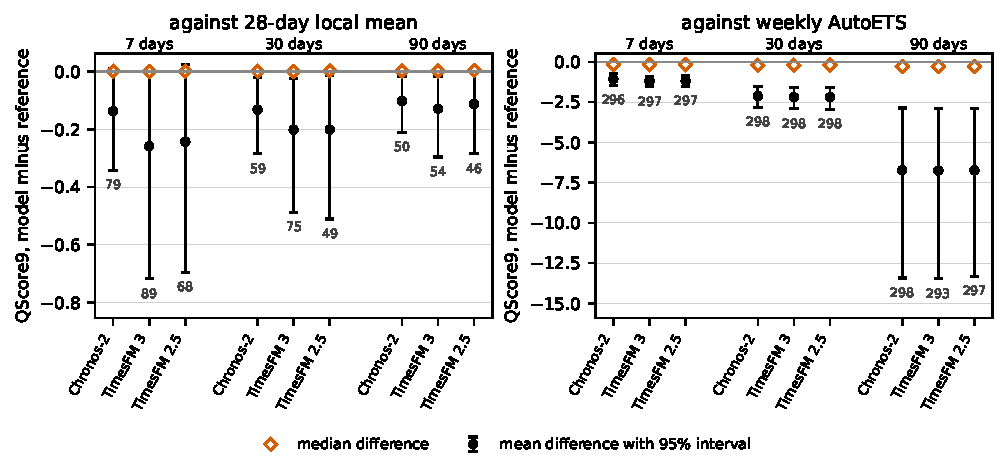
\includegraphics[width=\textwidth]{fig-paired-differences}
\caption{The 18 declared comparisons. Filled circles: mean difference (model minus reference \qs{}) with its
pointwise 95 percent repository-bootstrap interval. Open diamonds: median difference. The number under each
interval is the count of repositories, of 300, where the model's score is lower. Note the different vertical
scales.}
\label{fig:paired}
\end{figure}

\paragraph{Against the local mean.} In all nine cells the mean difference is negative, favoring the model,
from $-0.101$ (Chronos-2, 90 days) to $-0.258$ (TimesFM 3, 7 days), and the bootstrap interval excludes
zero in five cells: the three 30-day cells and the 90-day cells of Chronos-2 and TimesFM 3. The three 7-day
intervals and TimesFM 2.5 at 90 days include zero. In all nine cells the median difference is positive,
favoring the reference, and the model's score is lower on only 46 to 89 of the 300 repositories. The
signed-rank test rejects in all nine cells after adjustment (largest adjusted $p$ 0.0067, TimesFM 3 at 7
days); because every median is positive, the location shift the test detects favors the reference. The
signed-rank test is not a test of the mean, and the bootstrap interval is pointwise, not simultaneous; the
two statements do not contradict each other. The mean is carried by a minority of repositories with large
gains: in the declared scale review the five largest positive repository gains account for 88.5 to 94.3
percent of all positive gain against the local mean, and the leave-one-repository-out mean gain stays
positive in every cell (Appendix Table~\ref{tab:scale}). Ratio skill against the local mean is defined for
only 209, 239 and 259 of 300 repositories at 7, 30 and 90 days, because the reference's loss is zero on the
others; the report does not headline a ratio.

\paragraph{Against AutoETS.} In all nine cells both the mean and the median difference are negative, the
model's score is lower on 293 to 298 of 300 repositories, and the signed-rank test rejects in all nine; both
summaries favor the model. Mean differences grow with horizon, from $-1.07$ to $-1.19$ at 7 days to $-6.72$
to $-6.75$ at 90 days, and the 90-day intervals are wide. The reason is in the reference: AutoETS's nominal
80 percent intervals cover 98.6 to 98.8 percent of target days pooled over the panel (a declared secondary
summary), and in a width diagnostic requested after the run within that declared analysis its median 90-day
daily interval width is 0.79 stars per day in the smallest stratum, 3.60 in the middle one and 49.69 in the
top one (Appendix Table~\ref{tab:autoets}). Six fits at each horizon, from two repositories, selected
multiplicative seasonality, all in the top stratum; the specification counts were also requested after the
run. AutoETS is a weak uncertainty reference on this panel.

\paragraph{By stratum and calibration.} Pooled \qs{} by stratum (Appendix Table~\ref{tab:stratum}) holds
stratum means only: in the top stratum the three models' pooled scores are below the local mean's at every
horizon; in the smallest stratum the local mean's is below all three at every horizon; in the middle stratum
the four differ by less than 0.012 at every horizon; and AutoETS is far above all of them at every scale. The
typical repository by stratum is not in the declared tables. A post-hoc reading of the saved per-repository
accounting file, which adds no test, gives it: the median difference against the local mean is positive,
favoring the reference, in every stratum and every cell, and the models score lower on 5 to 18 of 100
repositories in the smallest stratum, 10 to 34 in the middle one and 26 to 38 in the top one. So the stratum
means and the typical repository disagree within the top stratum as the panel mean and the typical repository
disagree overall. Inclusive 80 percent coverage of the repaired deciles over the panel is 0.824 to 0.837 for
Chronos-2, 0.880 to 0.910 for TimesFM 3, 0.906 to 0.924 for TimesFM 2.5, 0.941 to 0.955 for the local mean
and 0.986 to 0.988 for AutoETS (Appendix Table~\ref{tab:calibration}). On discrete counts a correct quantile
can overcover \citep{czado2009}, so these are descriptive.


\section{Post-hoc accounting of the saved run}

This section is post-hoc. It was computed on 2026-09-14 from the saved forecasts after the registered
results were seen, adds no test, and does not change the status of anything above. Each window's \qs{} is
split exactly into three parts, each divided by the full horizon: the loss on zero-target days, which for
nonnegative quantiles is $\frac{2}{9h}\sum_{y_t = 0}\sum_\tau (1-\tau) q_{t,\tau}$; the loss on positive days
from quantiles above the target (overprediction); and the loss on positive days from quantiles below it
(underprediction). The parts sum to \qs{} on all 48,600 rows to floating-point tolerance, and the same
within-repository and across-repository averaging reproduces the 18 registered mean differences. The
decomposition locates where a loss difference arises; it says nothing about why a model forecast what it did.

\begin{table}[t]
\centering\small
\caption{Post-hoc. The mean difference against \lm{} and its three parts, model minus reference; negative
favors the model. The parts sum to the total.}
\label{tab:posthoc}
\begin{tabular}{llrrrr}
\toprule
Model & $h$ & Total & Zero days & Positive, overprediction & Positive, underprediction \\
\midrule
Chronos-2 & 7 & -0.137 & 0.005 & -0.095 & -0.048 \\
Chronos-2 & 30 & -0.132 & 0.005 & -0.156 & 0.019 \\
Chronos-2 & 90 & -0.101 & 0.004 & -0.184 & 0.078 \\
TimesFM 3 & 7 & -0.258 & 0.004 & -0.091 & -0.171 \\
TimesFM 3 & 30 & -0.201 & 0.006 & -0.150 & -0.057 \\
TimesFM 3 & 90 & -0.128 & 0.011 & -0.187 & 0.047 \\
TimesFM 2.5 & 7 & -0.243 & 0.012 & -0.088 & -0.167 \\
TimesFM 2.5 & 30 & -0.201 & 0.014 & -0.163 & -0.052 \\
TimesFM 2.5 & 90 & -0.112 & 0.015 & -0.209 & 0.082 \\
\bottomrule
\end{tabular}
\end{table}

Table~\ref{tab:posthoc} gives the parts for the nine cells against the local mean. The finding in one
sentence: the mean gain sits on positive days where the local mean overpredicts, and the zero-day part is
small beside it. The zero-day part is positive, against the models, in every cell, from 0.004 to 0.015: small
beside mean differences of $-0.101$ to $-0.258$, but in every cell larger than that cell's median
difference in Table~\ref{tab:lm}, where the medians run from 0.0003 to 0.0041. The overprediction part favors the models in every cell,
from $-0.088$ to $-0.209$. The underprediction part favors the models at 7 days, where for both TimesFM
models it is the larger of the two positive-day parts, and favors the local mean at 90 days, where the
models' underprediction loss exceeds the local mean's. Why the local mean overpredicts on those days is not
something the accounting tests.

\begin{figure}[t]
\centering
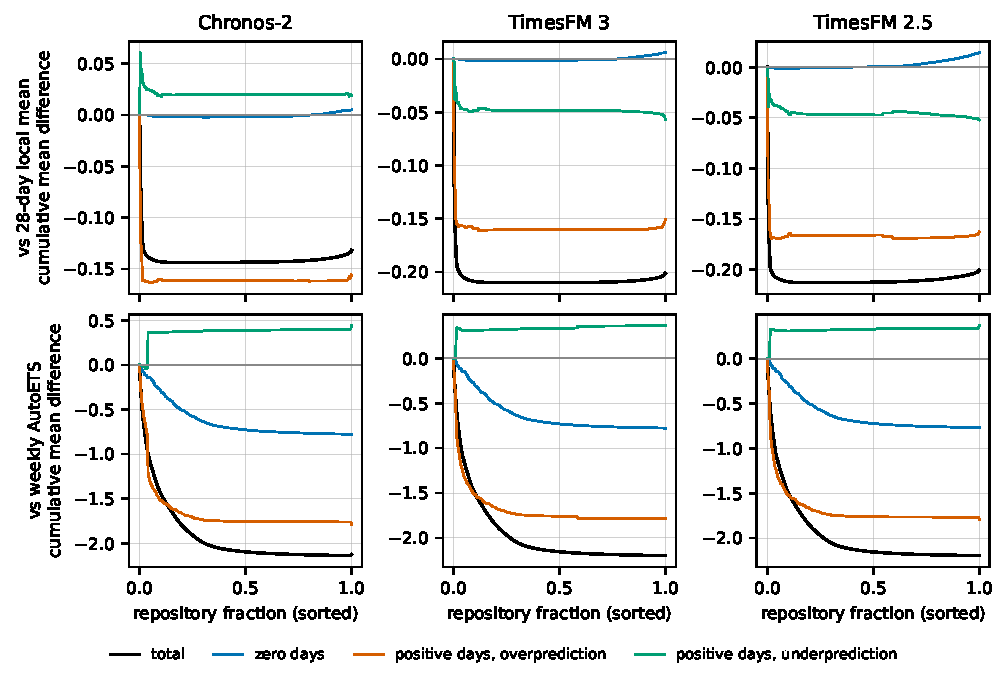
\includegraphics[width=\textwidth]{fig-posthoc-cumulative-h30}
\caption{Post-hoc. Signed cumulative contribution to the mean difference at horizon 30, repositories sorted
by their total difference (ascending) and the cumulative sum divided by 300, so each curve ends at its mean.
Top row: against \lm{}; bottom row: against \aets{}. Vertical scales differ between rows.}
\label{fig:cumulative}
\end{figure}

Figure~\ref{fig:cumulative} shows the same accounting as cumulative curves. Against the local mean, the total
drops to its final level within the first few percent of repositories and then drifts slightly upward over
the remaining majority, which lose by small amounts; against AutoETS the gain accrues across most of the
panel, and its largest part is overprediction on positive days, with a zero-day part between $-0.768$ and
$-0.777$. Appendix Figure~\ref{fig:zerofraction} places each repository by its context zero fraction: against
the local mean the large model gains are at low zero fractions and the small model losses cluster at high
ones, while against AutoETS nearly every repository at every zero fraction favors the model.


\section{Limitations}

\begin{itemize}
\item \emph{A fetch-time survivor panel.} The 470 skips were repositories that no longer resolved publicly in
  September 2026. Equal weighting describes the panel of repositories still public with complete histories,
  not all repositories created in the window.
\item \emph{Surviving stars, not gross additions.} The endpoint reports stars that still exist at retrieval.
  In the 2024 validation the endpoint total was below the archive total for 17 of 20 repositories; for the
  15 large projects the ratio ran from 0.728 to 0.994, with 13 of 15 at least 5 percent below. The study
  target is the surviving-star history; no correction is applied, and later unstars can change the apparent
  past.
\item \emph{Los Angeles day bins.} The endpoint's day boundary was resolved to America/Los\_Angeles days by
  validation, not documented by GitHub; the validation also showed that the transition days around daylight
  saving do not uniformly favor one calendar.
\item \emph{Three windows per repository, and horizons sharing targets.} Inference is conditional on the
  fixed calendar of three cutoffs; the 7- and 30-day targets are prefixes of the 90-day targets, so the
  nine cells per reference are not independent.
\item \emph{Pointwise intervals and BH.} The bootstrap intervals are pointwise, not simultaneous, and the
  Benjamini-Hochberg adjustment carries its usual dependence assumptions.
\item \emph{The signed-rank symmetry assumption.} The Wilcoxon test's location interpretation requires
  symmetric differences, which these are not; it is reported as registered and is not a test of the mean.
\item \emph{AutoETS as a weak uncertainty reference.} Its 80 percent intervals cover about 99 percent of
  target days; a model can beat it on nearly every repository by being less wide. Read with the coverage
  results, the comparison against the local mean is the more informative of the two; that is a reading made
  after the results, and both comparisons stay reported as registered.
\item \emph{Training contamination unresolved.} No author-disclosed complete-corpus training cutoff exists
  for any of the three models; the model cards name specific sources with dates, which do not bound the
  whole corpus. What can be said is bound by availability, per model. The targets, 2025-12-05 to 2026-08-31,
  postdate the pinned TimesFM 2.5 revision, dated 2025-10-02, but are not shown to postdate the pinned
  Chronos-2 revision, dated 2026-06-05, or the pinned TimesFM 3 revision, dated 2026-09-02 with weights
  uploaded 2026-08-24; these are repository revision dates, not training cutoffs. Every repository's history
  before the cutoffs may be familiar to all three models, and a later test window on familiar entities does
  not establish generalization to unseen ones \citep{moghadasi2026}. The controls are Study 1's registered
  follow-up cohort and the lapsed October holdout; neither has run (Section~\ref{sec:notrun}).
\item \emph{The mature-phase calendar.} Every repository is forecast between nine and 41 months after
  creation. Nothing here concerns launches or the days after a release.
\item \emph{Version 1 not recomputed.} The version 1 numbers are quoted from preserved documents.

\end{itemize}

\section{What is registered and not run}
\label{sec:notrun}

\paragraph{Study 1's follow-up cohort.} The protocol registers a separate follow-up on repositories created
on or after 2026-09-13, to run after this write-up with identical eligibility, strata, sample size, model
revisions, baselines, scores, regime rules and relative window calendar. It is an availability-bound
exclusion based on the already frozen checkpoints, not a claimed training cutoff; it contributes no test or
result to this report's family; and its creation-window closing date, future endpoint and frame coverage are
registered as still open, to be fixed before any follow-up collection. It has not run.


\paragraph{Study 2.} A second study of occurrence and positive size in daily count forecasts was registered
on 2026-09-14 as a dated addition at commit \texttt{df55867c982dfe2bb6e1152ec8ae93e3cd228c45} (full
protocol SHA-256 at registration
\texttt{33cefd8e34fea973e6747d1ba3fe565051e215c5d1b7f6553b266c1be7a66360}). It asks whether replacing a
foundation model's occurrence probability with a context-only estimate, while keeping its completed positive
conditional distribution, improves \qs{}, and whether that positive component improves on a fixed count
hurdle. The nearest published precedent applies an occurrence-times-size hurdle to frozen Chronos-2 output on
monthly spare-parts demand, judged by point and service measures \citep{chin2026}; the registered
construction, on daily counts under a proper score with a short-window occurrence estimate and matched
hurdles, has not been tested there. Study 2 declares 54 external tests over three domains (npm package
downloads, NYC 311 requests and Wikipedia pageviews, 300 series each in three context-zero-fraction strata),
6 synthetic tests on a seeded generator grid of 18 cells with 30 replicates, and 18 prospective tests on an
October 2026 calendar holdout over the frozen GitHub panel and an npm panel. Each family has one
Benjamini-Hochberg correction. As of 2026-10-12 no Study 2 target value, forecast or score existed; both
components fixed for the October 2026 paper, the synthetic grid and the npm external run, ran on 2026-10-15
and are reported in the paper that extends this report. Nothing is claimed here about their outcome.

\paragraph{The October holdout.} The holdout is Study 2's prospective component: a new calendar test on
possibly familiar entities, which the protocol says does not replace Study 1's follow-up cohort, and which
would not by itself show generalization to unseen entities \citep{moghadasi2026}. Its freeze deadline,
2026-09-28 18:00 UTC, passed with no freeze plan prepared, no forecast generated and no prediction committed.
Under the registered rule a late commit fails the prospective gate and no backdating is allowed. The dated
addition of 2026-10-12 to the protocol, committed at \texttt{8db0d73}, records the holdout as registered and
not run, resets the npm readiness clock once (a verified npm panel by 2026-10-20, else the registered PyPI
substitution), and declares that the external confirmatory family of the October 2026 paper is the eighteen
packages-domain tests E01 to E18 exactly as registered, with NYC 311 and Wikipedia deferred to a later family
of 36. The registered design had three external domains; two are not run before the paper.

\section{Reproducibility}

The repository \url{https://github.com/vprchlik/PulseGraph} contains the study code, the offline tests, the
protocol with its dated additions, the declarations under \texttt{study/} and the evidence package under
\texttt{reports/registered-2026-09-13/}, from the frozen manifest and daily signals to the confirmatory
inference tables and the post-hoc accounting; Appendix~\ref{app:repro} lists what it holds and does not hold,
the commands that regenerate every table, the hardware and package versions of the run, and the licences.
The complete results file \texttt{results.parquet} (433,172,286 bytes, SHA-256
\texttt{53ff5a5316fd43dd898866c4fc54edf913b080a32cbd696d7e3b3fc528f62df6}) holds every forecast, quantile
grid, context, target and seed. It is to be published as a GitHub release asset; the URL is to be filled by
the author at posting and is marked in the repository's README.


\section{How this work was made}

The following is the author's own statement, as it stands in the repository's README.

\begin{quote}
This study exists for three reasons: the question, whether zero-shot time-series foundation models improve
probabilistic forecasts of sparse daily counts; the audit of its first version, which found no invalidating
code defect but two design flaws; and the registered redesign that answers the question without them. The
code in this repository was written with AI coding agents under my direction. I set the question, registered
the protocol before any target data was fetched, ran the studies on my own machine, and made the decisions
that the protocol and the evidence package record as the author's. Every number in \texttt{RESULTS.md} traces
to a saved file under \texttt{reports/} and to the command that regenerates it, named in this README and in
\texttt{RESULTS.md}.
\end{quote}


\bibliographystyle{plainnat}
\bibliography{references}

\appendix

\section{The registered design, the remaining detail}
\label{app:design}

\paragraph{Count source and validation.} Daily counts come from GitHub's star-history endpoint
\citep{github-star-history-2026, github-api-star-history}, released 2026-09-04, from creation through the
common endpoint 2026-08-31. GH Archive supplies the frame, not the counts, because its WatchEvent capture
degraded from mid-2025 \citep{gharchive-issue-320}. Before the freeze, 20 validation repositories created
before 2023 (and so outside the study frame) were fetched and compared hourly with deduplicated GH Archive
WatchEvents over 2024. Over the 365 matched days, America/Los\_Angeles calendar days with daylight saving gave
the lowest mean absolute daily difference for 20 of 20 repositories against UTC and 18 of 20 against fixed
UTC$-$8, with two repositories tied between the Los Angeles and fixed-offset calendars (pooled mean absolute
difference 1.975 against 2.065 and 2.713); the author accepted Los Angeles days as the calendar. The endpoint
reports stars that still exist at retrieval, dated by when they were given: the 2024 endpoint total is below
the archive total for 17 of 20 repositories. The target is therefore the surviving-star daily history as
retrieved in September 2026, not gross additions.

\paragraph{Calendar.} The common endpoint $E$ is 2026-08-31. Cutoffs are $c_j = E - (j \times 90 - 1)$
days for $j = 3, 2, 1$: 2025-12-05, 2026-03-05 and 2026-06-03. Context ends the day before the cutoff;
targets run from the cutoff for 7, 30 or 90 days. The three 90-day windows partition the trailing 270 days
and do not overlap; shorter horizons use the same cutoffs, so horizons share targets and are not independent.
Every model has at least 90 context days, uses only the repository's own history, and refits (for the
baselines) on context only.

\paragraph{Regimes.} Three context-only labels, descriptive and pooled for inference: ``inactive recently''
when the 28 days before the cutoff sum to zero; ``recent surge'' when the last seven days hold at least seven
stars and their daily rate is at least three times the larger of the preceding four weeks' daily rate and one;
``other active'' otherwise. Tests perturb, permute and extend data on and after each cutoff and assert
unchanged labels and strata.

\paragraph{Models.} Three frozen foundation models with exact repository revisions:
\texttt{amazon/chronos-2} at \texttt{29ec3766d36d6f73f0696f85560a422f50e8498c} (weights and package
Apache-2.0) \citep{chronos2-weights, chronos2-2025};
\texttt{google/timesfm-3.0-pytorch} at \texttt{43046b85ec22d584a13f8098c2ed39c889e129c2} (weights under the
TimesFM Non-Commercial License v1.0, package Apache-2.0) \citep{timesfm3-card, timesfm-license};
\texttt{google/timesfm-2.5-200m-pytorch} at \texttt{1d952420fba87f3c6dee4f240de0f1a0fbc790e3} (Apache-2.0)
\citep{timesfm25-card}. All run univariate, batch size one, a 2,048-day maximum context, on one GPU. Two
primary references: \lm{}, the mean of the last 28 context days with 200 empirical context-level draws, and
\aets{}, StatsForecast AutoETS with season length 7 and native intervals \citep{statsforecast-2.1.1}. Thirteen
secondary baselines: AutoARIMA and AutoTheta with weekly season, a negative-binomial local level with a 28-day
mean and context-moment dispersion, local means with lookbacks 7, 14, 56 and 90, and the version 1 families
(last value, weekly naive, horizon-dependent seasonal naive, 30-day linear trend, nonseasonal Holt, LightGBM).

\paragraph{Score.} The primary score is \qs{}, twice the mean pinball loss over the nine deciles
$\tau \in \{0.1, \dots, 0.9\}$ and the $h$ target days,
\[
\qs{} = \frac{2}{9h} \sum_{t=1}^{h} \sum_{\tau} \max\{\tau (y_t - q_{t,\tau}),\, (\tau - 1)(y_t - q_{t,\tau})\},
\]
defined for all-zero targets and equal to the weighted interval score at the matching levels
\citep{bracher2021}; it is a proper score for the nine quantiles \citep{gneiting2007}. Deciles are native or
analytic where a model supplies them and linear empirical quantiles of 200 draws otherwise; negative
forecasts are clipped to zero and crossings repaired by cumulative maxima, with both repairs recorded. No
tails beyond the supported deciles are invented for either TimesFM.

\paragraph{Inference.} Window scores are averaged within repository and horizon, then repositories are
weighted equally. For each of the 18 declared comparisons (three models, two references, three horizons)
the paired difference $d$ is model minus reference, so negative favors the model. The mean of $d$ carries a
pointwise 95 percent percentile interval from 20,000 bootstrap replicates of whole repositories (seed
20260914). A two-sided approximate Wilcoxon signed-rank test across repository averages, omitting zero
differences, tests a zero-centered symmetric null; its location interpretation requires symmetry and it is
not a test of the mean. Benjamini-Hochberg adjustment is applied once at $q = 0.05$ over the 18 tests, with
its usual dependence assumptions. Strata, regimes, other lookbacks, calibration and the scale review are
declared secondary and add no test. Seeds: selection 20260913, forecast 20260912, bootstrap 20260914.


\section{Version 1: the disclosure list and the local-mean table}
\label{app:v1}

The audit listed what version 1 had to disclose: a weak original baseline set; Wilcoxon tests on overlapping
windows treated as independent; untested scale domination; a mislabeled 95 percent interval for TimesFM,
whose API exposes only the 0.1 to 0.9 quantiles; ordinary PIT on discrete counts; unseeded baseline sampling;
LightGBM's uncertainty from in-sample residuals; MAPE as a headline metric on zero-inflated series; implicit
observation endpoints that censored trailing zeros and omitted later-removed stars; and unresolved
pretraining contamination with no clean post-release holdout. Every version 1 number in this report is
quoted from the preserved version 1 documents (its results document, its audit and its write-up, with four
figures), not recomputed. The version 1 result artifacts (the results parquet, the summary CSV, the review
outputs and the raw stargazer data) were excluded from that repository by its ignore rules and exist only on
a computer the author no longer uses; their recovery is deferred.

\begin{table}[h]
\centering\small
\caption{Version 1, quoted from the preserved documents: mean CRPS of the 28-day local mean added by the
audit and of the two foundation models, by discovery cohort and horizon. These numbers were not recomputed;
the version 1 artifacts are on a computer the author no longer uses.}
\label{tab:v1}
\begin{tabular}{llrrr}
\toprule
Cohort & Horizon (days) & Local mean & Chronos-2 & TimesFM-2.5 \\
\midrule
breakout-selected & 7 & 7.77 & 6.43 & 6.23 \\
breakout-selected & 30 & 8.77 & 7.90 & 7.68 \\
breakout-selected & 90 & 9.41 & 8.52 & 8.20 \\
steady-selected & 7 & 1.66 & 1.46 & 1.44 \\
steady-selected & 30 & 2.26 & 2.04 & 2.02 \\
steady-selected & 90 & 2.42 & 2.21 & 2.22 \\
dead-selected & 7 & 2.75 & 2.43 & 2.35 \\
dead-selected & 30 & 2.64 & 2.47 & 2.39 \\
dead-selected & 90 & 2.85 & 2.73 & 2.67 \\
\bottomrule
\end{tabular}
\end{table}


\section{Reproducibility, the detail}
\label{app:repro}

\paragraph{What a fresh clone holds.} The repository contains the study code, the offline tests, the
protocol with its dated additions, the declarations under \texttt{study/} (the 18 comparisons, the run
specification with model revisions, the 20 validation repositories, both SQL queries), and the evidence
package under \texttt{reports/registered-2026-09-13/}: the frozen manifest and aggregate daily signals, the
full eligible frame and its frozen order, the skip log, the query exports and provenance, the hourly
validation comparison and figures, the signed readiness review, the run metadata with package versions and
hardware, the integrity log, the confirmatory inference tables, the declared descriptive tables and the
post-hoc accounting. It does not contain raw endpoint responses, model weights, the version 1 reference copy,
or the private research notes. The BigQuery frame and validation queries billed 12,510,623,170,560 bytes
(about \$71.11 at the list price before credits), approved in writing before they ran.

\paragraph{Commands.} Place the release asset at
\texttt{reports/registered-2026-09-13/run/results.parquet}, then from the repository root, with the
project's Python environment:
{\footnotesize
\begin{verbatim}
.\.venv\Scripts\python.exe -m scripts.review_integrity --run reports/registered-2026-09-13/run
.\.venv\Scripts\python.exe -m scripts.registered_inference --run reports/registered-2026-09-13/run `
    --out data/cache/inference-reproduction
.\.venv\Scripts\python.exe reports/registered-2026-09-13/summarize_descriptives.py
\end{verbatim}}
The first verifies hashes, the grid, contexts, targets, labels, seeds and recomputes every score; the second
regenerates the 18-row inference table from the saved forecasts without refitting; the third regenerates the
descriptive CSVs behind the tables of Appendix~\ref{app:tables}. The post-hoc accounting is regenerated by
\texttt{reports/registered-2026-09-13/posthoc/accounting.py}, and the figures of this report by
\texttt{paper/figures/make\_figures.py}, which reads only the saved CSVs. The run itself used an NVIDIA
GeForce RTX 4070 SUPER (driver 610.47, CUDA 12.8, PyTorch 2.11.0), \texttt{chronos-forecasting} 2.3.2,
\texttt{timesfm} 3.0.2 and \texttt{statsforecast} 2.1.1 \citep{timesfm-pypi, statsforecast-2.1.1}.

\paragraph{Licences.} The code is MIT. The aggregate dataset and this write-up are CC BY 4.0. Chronos-2 and
TimesFM 2.5 weights are Apache-2.0; TimesFM 3 weights carry the TimesFM Non-Commercial License v1.0; the
Chronos and TimesFM packages are Apache-2.0.


\section{Additional tables and figure}
\label{app:tables}

\begin{table}[h]
\centering\small
\caption{AutoETS interval coverage and 90-day widths by stratum. Coverage is a declared secondary summary:
inclusive coverage of the repaired 0.1 to 0.9 quantiles at each horizon. The widths and the specification
counts were requested after the run, within the declared secondary calibration analysis. Widths are the
median over fits of the 90-day daily width and the median of the fit-mean width, both after clipping and
crossing repair. The last column counts fits that selected multiplicative seasonality, at each horizon.}
\label{tab:autoets}
\begin{tabular}{lrrrrrr}
\toprule
Stratum & Cov.\ $h=7$ & $h=30$ & $h=90$ & Daily width & Fit-mean width & Mult.\ fits \\
\midrule
20--99 & 0.979 & 0.978 & 0.980 & 0.79 & 0.80 & 0 \\
100--999 & 0.991 & 0.988 & 0.989 & 3.60 & 3.71 & 0 \\
1000+ & 0.991 & 0.994 & 0.995 & 49.69 & 55.99 & 6 \\
\bottomrule
\end{tabular}
\end{table}

\begin{table}[h]
\centering\small
\caption{Pooled \qs{} by day-90 stratum and horizon, declared secondary: three windows averaged within
repository, then 100 repositories per stratum weighted equally. These are stratum means; the typical
repository by stratum is given, labeled post-hoc, in Section~\ref{sec:results}.}
\label{tab:stratum}
\begin{tabular}{llrrrrr}
\toprule
Stratum & $h$ & Chronos-2 & TimesFM 3 & TimesFM 2.5 & \lm{} & \aets{} \\
\midrule
20-99 & 7 & 0.077 & 0.077 & 0.079 & 0.075 & 0.148 \\
20-99 & 30 & 0.084 & 0.084 & 0.085 & 0.082 & 0.162 \\
20-99 & 90 & 0.086 & 0.101 & 0.088 & 0.083 & 0.189 \\
100-999 & 7 & 0.217 & 0.219 & 0.226 & 0.228 & 0.542 \\
100-999 & 30 & 0.217 & 0.215 & 0.221 & 0.217 & 0.703 \\
100-999 & 90 & 0.233 & 0.231 & 0.235 & 0.236 & 0.967 \\
1000+ & 7 & 2.798 & 2.432 & 2.470 & 3.200 & 5.609 \\
1000+ & 30 & 3.134 & 2.929 & 2.923 & 3.531 & 8.950 \\
1000+ & 90 & 3.966 & 3.874 & 3.930 & 4.270 & 23.301 \\
\bottomrule
\end{tabular}
\end{table}

\begin{table}[h]
\centering\small
\caption{Inclusive 80 percent coverage of the repaired 0.1 to 0.9 quantiles, averaged within repository and
then over 300 repositories, declared secondary.}
\label{tab:calibration}
\begin{tabular}{lrrr}
\toprule
Model & $h=7$ & $h=30$ & $h=90$ \\
\midrule
chronos2 & 0.832 & 0.824 & 0.837 \\
timesfm3 & 0.880 & 0.910 & 0.889 \\
timesfm2p5 & 0.924 & 0.906 & 0.918 \\
local\_mean\_28 & 0.955 & 0.945 & 0.941 \\
autoets\_weekly & 0.987 & 0.986 & 0.988 \\
\bottomrule
\end{tabular}
\end{table}

\begin{table}[h]
\centering\small
\caption{The declared scale review against \lm{}. The top-five share divides the five largest positive
repository gains (reference minus model) by all positive gains. Skill, $1 - \text{model}/\text{reference}$,
is undefined where the reference's loss is zero. The leave-one-out range is the mean gain with each
repository removed in turn.}
\label{tab:scale}
\begin{tabular}{llrrc}
\toprule
Model & $h$ & Top-five share of positive gain & Skill defined (of 300) & Leave-one-out mean gain \\
\midrule
Chronos-2 & 7 & 0.902 & 209 & [0.060, 0.152] \\
Chronos-2 & 30 & 0.910 & 239 & [0.074, 0.134] \\
Chronos-2 & 90 & 0.892 & 259 & [0.068, 0.105] \\
TimesFM 3 & 7 & 0.932 & 209 & [0.066, 0.280] \\
TimesFM 3 & 30 & 0.929 & 239 & [0.083, 0.203] \\
TimesFM 3 & 90 & 0.895 & 259 & [0.064, 0.133] \\
TimesFM 2.5 & 7 & 0.943 & 209 & [0.049, 0.265] \\
TimesFM 2.5 & 30 & 0.943 & 239 & [0.073, 0.203] \\
TimesFM 2.5 & 90 & 0.885 & 259 & [0.046, 0.120] \\
\bottomrule
\end{tabular}
\end{table}

\begin{figure}[h]
\centering
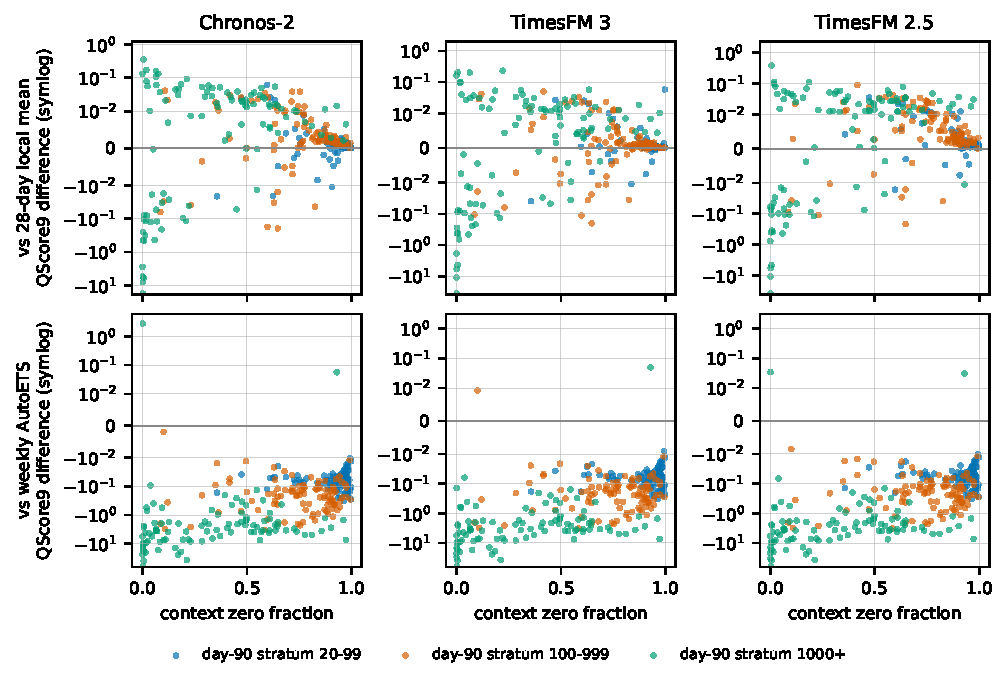
\includegraphics[width=\textwidth]{fig-posthoc-zero-fraction-h30}
\caption{Post-hoc. Each repository's paired difference at horizon 30 against the fraction of zero days in
its context (three windows averaged), colored by day-90 stratum, on a symmetric log scale. Top row: against
\lm{}; bottom row: against \aets{}. Against the local mean the large model gains are at low zero fractions
and the small model losses cluster at high ones; against AutoETS nearly every repository at every zero
fraction favors the model.}
\label{fig:zerofraction}
\end{figure}


\end{document}
